\chapter{Definición del Problema y Análisis}

\section{Formulación del Problema}

Utilice el problema expuesto en el documento de propuesta, incluyendo las observaciones entregadas por su profesor Guía. Por otra parte, intente contrastar lo detectado con diferentes fuentes. 

\section{Solución Propuesta}

Considerando los hallazgos de la etapa anterior y de ésta presente la solución propuesta. Por otra parte, considere exponer el impacto que ésta tendrá, ya sea social, comercial, académico u otro. 

\section{Objetivos}
En un buen objetivo es posible identificar los siguientes elementos:
\begin{itemize}
    \item Qué: Qué realizaré. 
    \item Cómo: Cómo espero realizarlo (ej: tecnología). 
    \item Para qué: Por qué es necesario realizarlo. 
\end{itemize}

Además, los objetivos específicos deben ser consistentes con el objetivo general, y asegurar el alcanzarlo.

\subsection{Objetivo General}
\label{sc:OG}

\subsection{Objetivos Específicos}
\label{ssc:OE}

\section{Metodología}
\label{sc:Met}

Se debe evidenciar coherencia entre la opción metodológica, el problema y los objetivos planteados.
Por otra parte, la realización de un esquema facilita la comprensión de su opción metodológica. Para finalizar, considere los tiempos de seminario de título al momento de definir una metodología.


En la Figura \ref{fig:met}, se presenta cómo insertar una imagen en \LaTeX{}.
\begin{figure}[H]
    \centering
    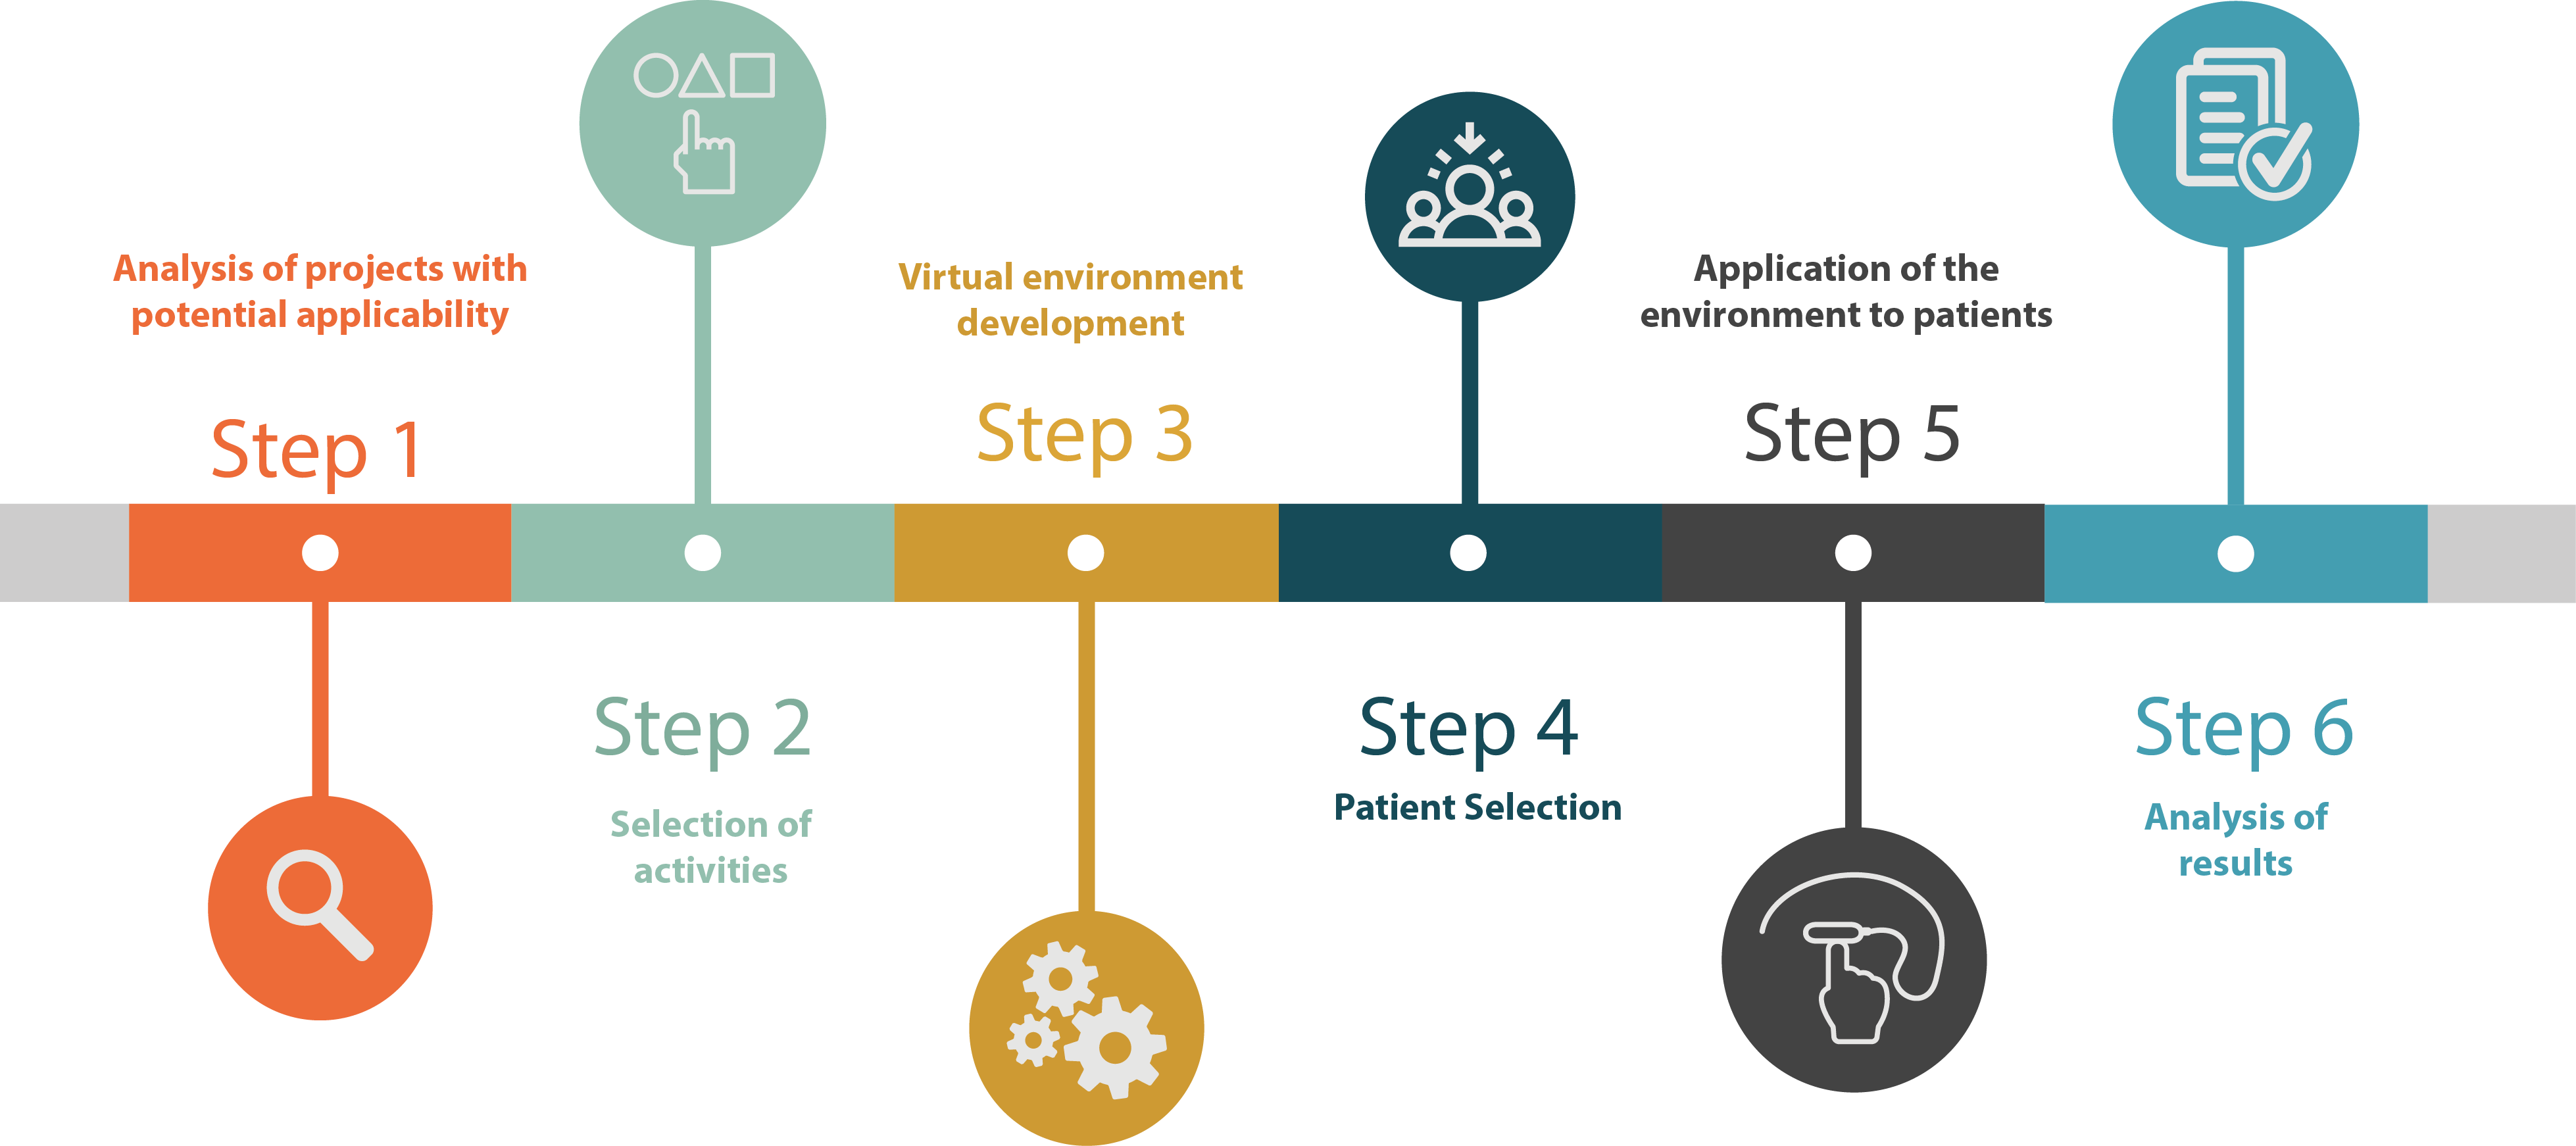
\includegraphics[width=0.75\textwidth]{imagenes/Fig_ejMet.png}
    \caption{Ejemplo de como insertar una figura}
    \label{fig:met}
\end{figure}



\section{Especificación de Requerimientos}
\label{sc:ER}


\subsection{Requerimientos Funcionales}
\label{ssc:RF}


\subsection{Requerimientos No Funcionales}
\label{ssc:RNF}
\section{Funcionalidades del Sistema}
\label{sc:FS}


\subsection{Diagramas de Casos de Uso}
\label{ssc:DCU}


\subsection{Casos de Uso}
\label{ssc:CU}

\subsection{Diagramas de Secuencia}
\label{ssc:DSS}

\subsection{Diagramas de Estado}
\label{ssc:DE}


\subsection{Modelo Conceptual}
\label{ssc:MC}